\documentclass[a4paper]{article}
\usepackage {changepage}
\usepackage{fancyhdr}
\usepackage {fontspec}
\usepackage {paralist}
\usepackage {multicap}
\pagestyle{fancy}
\setromanfont{Lantinghei SC Extralight}
\setmonofont{Courier New}
\XeTeXlinebreaklocale ``zh''
\XeTeXlinebreakskip = 0pt plus 1pt
\textheight = 650pt
\begin{document}
\title{实验报告 Lab 7}
\author{姓名:王钦\quad 学号:13349112}
\date{}
\maketitle

\section*{  Capturing and analyzing Ethernet frames}
\hangindent=4em \hangafter=-200{
\begin{enumerate}
		\item My address:\verb| 84:38:35:68:46:ea|
			\begin{center} 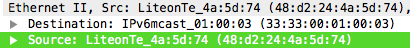
\includegraphics[scale=0.5]{Illustrations/1.png} \mfcaption{ethernet frame}\end{center}
		\item destination address:\verb| b0:48:7a:41:45:46|,isn't the Ethernet address of gaia.cs.umass.edu. 
		  This is the address of my router, the link is used to depart off the subnet.
		\item 0x0086 
		\item it's 52 bytes from the start. 
		\item 
		\item source address:\verb| b0:48:7a:41:45:46|
			\begin{center} 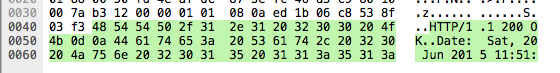
\includegraphics[scale=0.5]{Illustrations/2.png} \mfcaption{ethernet frame}\end{center}
			,isn't the Ethernet address of gaia.cs.umass.edu. 
		  This is the address of my router, the link is used just get in my subnet.
		\item destination address:\verb| 84:38:35:68:46:ea|,this is my address.	
		\item 0x0086 
		\item it's 52 bytes from the very start of the ethernet frame.
			\begin{center} 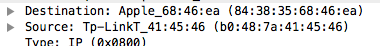
\includegraphics[scale=0.5]{Illustrations/3.png} \mfcaption{ethernet frame}\end{center}
		\item \ 

	    \newcounter{enumTemp}\setcounter{enumTemp}{\theenumi}
\end{enumerate}
}

\section*{ The Address Resolution Protocol}
\hangindent=4em \hangafter=-200{
	\begin{enumerate}
		\setcounter{enumi}{\theenumTemp}
		\item first column mean the IP address, the second column mean the MAC address, and the third column mean the adapter card. 
			\begin{center} 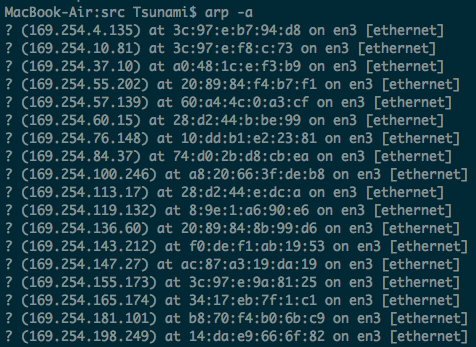
\includegraphics[scale=0.5]{Illustrations/4.png} \mfcaption{ARP Caching}\end{center}
		\item source address:\verb| 70:3e:ac:37:67:71|,destination address:\verb| 86:38:35:86:8e:64|.
			\begin{center} 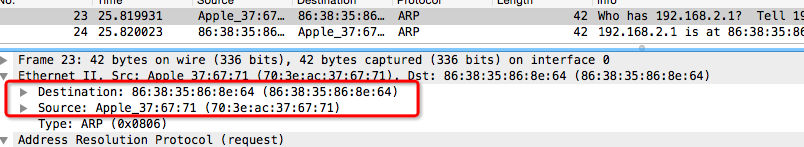
\includegraphics[scale=0.5]{Illustrations/5.png} \mfcaption{ARP Caching}\end{center}
		\item \verb|0x0806|.
		\item ARP request
		  \begin{enumerate}[a]
			\item it's 20 bytes from the very beginning of the Ethernet frame 
			  \begin{center} 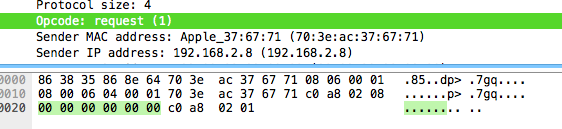
\includegraphics[scale=0.5]{Illustrations/6.png} \mfcaption{ARP Caching}\end{center}
			\item the value of opcode field is 1
			\item Yes, it containg the IP address \verb|192.168.2.8| which is sender.  
			  \begin{center} 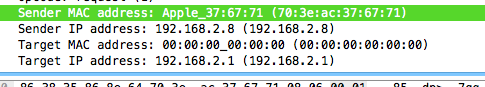
\includegraphics[scale=0.5]{Illustrations/7.png} \mfcaption{ARP Caching}\end{center}
			\item The of of \verb|Target MAC address| is \verb|00:00:00:00:00:00| mean address \verb|192.168.2.1| is queried. 
		  \end{enumerate}
		\item  ARP replay
		  \begin{enumerate}[a]
			\item it's 20 bytes from the very beginning of the Ethernet frame 
			  \begin{center} 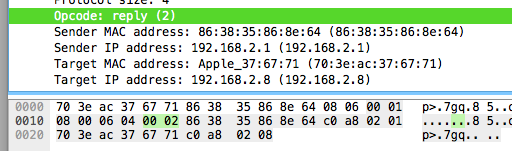
\includegraphics[scale=0.5]{Illustrations/8.png} \mfcaption{ARP Caching}\end{center}
			\item the value of opcode field is 2
			\item The answer to the earlier ARP request appears in the \verb|send MAC address|,the value \verb|86:38:35:86:8e:64| is the MAC address of 
			  \verb|192.168.2.1|
			  \begin{center} 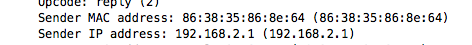
\includegraphics[scale=0.5]{Illustrations/9.png} \mfcaption{ARP Caching}\end{center}
		  \end{enumerate}
		\item source address:\verb| 86:38:35:86:8e:64|,destination address:\verb| 70:3e:ac:37:67:71|.
			  \begin{center} 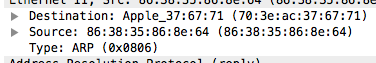
\includegraphics[scale=0.5]{Illustrations/10.png} \mfcaption{ARP Caching}\end{center}
		\item We can't receive this reply.Because ARP reply is sent back directly not broadcast.Only that send computer could receive the reply.

	\end{enumerate}
}
\end{document}




